\documentclass[11pt,a4paper]{article}

\usepackage[utf8]{inputenc}
\usepackage[T1]{fontenc}
\usepackage{lmodern}
\usepackage[french]{babel}
\usepackage{csquotes}
\usepackage{geometry}
\usepackage{booktabs}
\usepackage{longtable}
\usepackage{array}
\usepackage{enumitem}
\usepackage{graphicx}
\usepackage{xcolor}
\usepackage{hyperref}
\usepackage[backend=biber,style=authoryear,sorting=nyt]{biblatex}

\geometry{margin=2.5cm}
\setlength{\parskip}{0.65em}
\setlength{\parindent}{0pt}
\setlist[itemize]{leftmargin=1.2cm}
\setlist[enumerate]{leftmargin=1.2cm}
\renewcommand{\arraystretch}{1.2}
\graphicspath{{docs/c4/}{c4/}}

\hypersetup{
  colorlinks=true,
  linkcolor=blue,
  citecolor=blue,
  urlcolor=blue,
  pdftitle={RAGnos : assistant RAG medical pour l'information en reanimation},
  pdfauthor={Projet RAGnos}
}

\addbibresource{rapport_ragnos_juridique.bib}

\title{\textbf{RAGnos : assistant conversationnel RAG pour l'information en reanimation}\\
\large Rapport de projet}
\author{Projet RAGnos}
\date{5 juin 2026}

\begin{document}

\maketitle

\begin{abstract}
Ce rapport presente la reorientation de RAGnos vers un assistant documentaire medical centre sur la reanimation. Le besoin n'est plus la consultation juridique, mais l'information prudente, sourcee et comprehensible des proches de patients hospitalises en service de reanimation. Le prototype vise a interroger un corpus local compose de PDF medicaux et de transcriptions de videos pedagogiques, puis a produire des reponses ancrees dans ces documents. Il ne pose pas de diagnostic, ne prescrit pas et ne remplace pas l'equipe soignante. Les assistants medicaux disponibles visent principalement les cliniciens, tandis que les societes savantes proposent surtout des ressources pedagogiques destinees aux patients et a leurs proches \autocite{uptodateExpertAI,clinicalKeyAI,dynaAI,openEvidence,doximityAsk,sccmPatientFamilyResources,esicmPatientFamily,icsPatientResources}. RAGnos se positionne donc comme un prototype local, transparent et limite, centre sur la pedagogie securisee.
\end{abstract}

\tableofcontents
\newpage

\section{Introduction}

L'hospitalisation en reanimation est une situation de grande vulnerabilite pour les patients et leurs proches. Les patients peuvent etre sedates, intubes, dialyses, surveilles en continu ou places sous assistance d'organe. Pour les familles, l'environnement technique est souvent difficile a comprendre : respirateur, scope, pousse-seringues, dialyse, sedation, nutrition artificielle, soins de confort, limitations de traitement ou fin de vie. Les proches disposent surtout des equipes soignantes pour comprendre la situation et poser leurs questions.

Le projet RAGnos repond a ce besoin d'explication documentaire. L'objectif n'est pas d'automatiser la relation medicale, mais de fournir une interface locale capable d'expliquer des notions generales a partir d'un corpus valide : guides de societes savantes, brochures patients, recommandations, PDF institutionnels et transcriptions de videos pedagogiques. Les ressources francaises de la SFAR et de la SRLF documentent deja l'information aux patients de reanimation et a leurs proches, la place des visites et la necessite d'une communication simple et prudente \autocite{sfarInfoPatientsRea,srlfVisitesProches}.

La generation augmentee par la recherche (\emph{Retrieval-Augmented Generation}, RAG) est pertinente dans ce contexte parce qu'elle impose un ancrage documentaire : le modele ne doit pas repondre librement a partir de sa memoire interne, mais a partir de passages recuperes dans le corpus local. Cette approche ne supprime pas le risque d'erreur. Elle le rend cependant plus maitrisable, car les sources peuvent etre affichees, evaluees, remplacees et testees.

\section{Besoin metier en reanimation}

\subsection{Public cible}

Le public principal n'est pas le clinicien expert, mais le proche d'un patient hospitalise. Cette distinction est structurante. Un assistant destine aux proches doit eviter le jargon, expliquer progressivement, accepter l'incertitude, separer l'information generale du cas individuel et renvoyer vers l'equipe soignante lorsqu'une question concerne l'etat precis d'un patient.

Les recommandations sur les soins centres sur la famille mettent notamment en avant la presence et l'implication des proches, une information structuree, des supports educatifs, la communication autour de l'incertitude, le soutien psychologique et l'attention aux situations de fin de vie \autocite{sccmFamilyCentered2024}. Les ressources francaises de la SFAR et de la SRLF insistent egalement sur la necessite d'une information simple, adaptee aux familles, et sur la place centrale de l'equipe medicale dans les decisions \autocite{sfarInfoPatientsRea,srlfVisitesProches}.

\subsection{Fonctions attendues}

Pour ce projet, les fonctions utiles ne sont pas celles d'un outil d'aide au diagnostic. Les fonctions defendables sont plus modestes :

\begin{itemize}
  \item expliquer le vocabulaire courant de reanimation ;
  \item resumer une procedure generale de soin ou d'assistance d'organe ;
  \item orienter vers les sources utilisees ;
  \item rappeler les limites entre information generale et situation individuelle ;
  \item refuser lorsqu'une information n'est pas presente dans les documents ;
  \item aider les proches a formuler des questions a poser aux soignants.
\end{itemize}

Ce cadrage est important juridiquement et cliniquement. L'orientation \enquote{information generale, non diagnostique, non prescriptive} limite le risque d'assimilation a un dispositif medical ou a un outil de decision clinique ; cette delimitation doit etre examinee au regard des cadres reglementaires applicables \autocite{fdaGenAILifecycle,euAIActHealthcare}.

\section{Etat du marche}

\subsection{Un marche surtout clinicien}

Le marche des assistants medicaux fondes sur corpus est deja actif, mais il vise principalement les professionnels de sante. UpToDate Expert AI, ClinicalKey AI, Dyna AI, OpenEvidence et Doximity Ask se positionnent autour de la decision clinique, de la recherche de preuves, de la synthese de recommandations ou de la consultation rapide au point of care \autocite{uptodateExpertAI,clinicalKeyAI,dynaAI,openEvidence,doximityAsk}.

Ces solutions ont une force evidente : elles s'appuient sur des corpus maintenus, editorialisés ou relies a la litterature biomedicale. En revanche, elles ne repondent pas directement au besoin des proches en reanimation. Leur public cible reste le clinicien, leur langage peut etre technique, leur architecture est souvent partiellement publique ou opaque, et leur valeur repose sur des corpus proprietaires.

\subsection{Solutions proches du besoin famille}

Pour les patients et les familles, les solutions identifiees sont surtout des ressources d'education : pages institutionnelles, livrets, videos, FAQ, applications de communication ou journaux de reanimation. La SCCM propose des ressources patients/familles et une application de communication patient-famille-soignant ; l'ESICM, l'Intensive Care Society, ICUsteps, des hopitaux et les societes savantes francaises proposent aussi des contenus pedagogiques \autocite{sccmPatientFamilyResources,esicmPatientFamily,icsPatientResources,sfarInfoPatientsRea,srlfVisitesProches}.

Les ressources disponibles pour les patients et les familles sont principalement documentaires et pedagogiques \autocite{sccmPatientFamilyResources,esicmPatientFamily,icsPatientResources,sfarInfoPatientsRea,srlfVisitesProches}. RAGnos vise a les rendre plus accessibles dans une interface conversationnelle documentee, sans se substituer a l'equipe soignante.

\begin{longtable}{p{2.7cm}p{2.9cm}p{3.8cm}p{3.7cm}}
\caption{Positionnement des solutions proches d'un assistant RAG medical}\\
\toprule
\textbf{Solution ou categorie} & \textbf{Cible} & \textbf{Forces} & \textbf{Limites pour RAGnos}\\
\midrule
\endfirsthead
\toprule
\textbf{Solution ou categorie} & \textbf{Cible} & \textbf{Forces} & \textbf{Limites pour RAGnos}\\
\midrule
\endhead
UpToDate Expert AI & Cliniciens & Corpus medical maintenu, logique de reponse ancree dans du contenu expert. & Produit proprietaire, cible point of care, peu adapte aux proches. \\
ClinicalKey AI & Cliniciens & RAG medical publicise, cadre d'evaluation clinique multidimensionnel. & Usage professionnel, corpus ferme, faible transparence fine du pipeline. \\
Dyna AI / DynaMed & Cliniciens & Methodologie evidence-based, mise a jour editoriale continue. & Orientation decision clinique plutot qu'information famille. \\
OpenEvidence & Medecins, chercheurs & Acces rapide a la litterature biomedicale avec citations. & Langage technique, architecture opaque, inadapte comme outil famille. \\
Doximity Ask & Cliniciens & Liens vers guidelines, tables et journaux. & Public professionnel, transparence limitee. \\
Ressources SCCM, ESICM, SFAR, SRLF, ICS & Patients et proches & Pedagogie, information generaliste, vocabulaire ICU, place des familles. & Ressources dispersees, rarement conversationnelles. \\
\bottomrule
\end{longtable}

\section{Etat de l'art RAG medical}

\subsection{Retrieval hybride et reranking}

Les travaux MIRAGE / MedRAG montrent l'interet de combiner plusieurs corpus et plusieurs strategies de retrieval ; les configurations fortes associent recherche lexicale, recherche dense biomedicale et fusion de resultats \autocite{mirageMedrag}. Cette conclusion est coherente avec le besoin de RAGnos : une question de proche peut etre conceptuelle (\enquote{a quoi sert la sedation ?}) ou tres lexicale (\enquote{qu'est-ce que l'ECMO ?}).

Le reranking est egalement important. Un premier retrieval peut ramener trop de passages ou des passages proches mais imparfaits. Un reranker permet de reordonner les candidats avant generation, ce qui reduit le risque d'utiliser un contexte mal cible. RAGnos implemente aujourd'hui une recherche vectorielle simple ; la recherche hybride et le reranking constituent donc des evolutions prioritaires.

\subsection{Chunking et metadonnees}

Les documents medicaux longs posent un probleme de decoupage. Un chunking fixe peut separer une recommandation de son contexte, une indication de sa contre-indication, ou un tableau de son titre. Dans un corpus de reanimation, cette difficulte est accentuee par la diversite des sources : PDF de recommandations, brochures, formulaires, transcripts de videos, textes reglementaires et guides familles.

Les metadonnees doivent donc devenir une brique de fiabilite : type de source, public cible, date, societe savante, theme medical, niveau de preuve, pays, langue, statut de validation. Pour RAGnos, les fichiers JSON de transcripts fournissent deja des champs utiles (\texttt{title}, \texttt{author}, \texttt{topic}, \texttt{source\_type}, \texttt{url}). Le pipeline a ete adapte pour les conserver dans les documents indexes.

\subsection{Grounding, citations et refus}

En medecine, une reponse sourcee ne suffit pas si la source ne supporte pas precisement l'affirmation. MedRAGChecker propose d'evaluer la \emph{groundedness} par decomposition en affirmations et verification de leur support dans les passages recuperes \autocite{medRAGChecker}. En cas d'ancrage insuffisant, le systeme doit refuser de repondre ou fournir une reponse de repli.

RAGnos ajoute deja un bloc \texttt{Sources:} de maniere deterministe a partir des metadonnees recuperees. C'est preferable a une citation generee librement par le modele. La prochaine etape serait de lier les citations aux phrases de la reponse ou d'ajouter un seuil de pertinence minimal avant generation.

\section{Corpus et sources}

\subsection{Sources a privilegier}

Le corpus cible doit privilegier des sources institutionnelles et cliniques validees, notamment les ressources des societes savantes de reanimation \autocite{sccmPatientFamilyResources,esicmPatientFamily,icsPatientResources,sfarInfoPatientsRea,srlfVisitesProches} :

\begin{itemize}
  \item societes savantes de reanimation et soins critiques : SRLF, SFAR, SCCM, ESICM ;
  \item ressources patients et proches : brochures, FAQ, videos pedagogiques, livrets ICU ;
  \item recommandations sur les visites, la communication, la fin de vie et les soins palliatifs en ICU ;
  \item documents HAS sur le syndrome post-reanimation ;
  \item supports hospitaliers patients/familles clairement identifies.
\end{itemize}

La valeur du prototype dependra moins du modele que de la qualite de ce corpus. Un assistant local peut etre plus transparent et mieux adapte a la langue francaise qu'un produit generaliste, mais il ne peut pas compenser un corpus incomplet, obsolescent ou mal annote.

\subsection{Corpus actuel}

Le corpus actuellement exploitable combine des documents PDF institutionnels et des transcriptions de videos pedagogiques. Il couvre les grandes questions que se posent les proches : assistance respiratoire, assistance cardiaque et circulatoire, assistance renale, nutrition artificielle, sedation, surveillance, nursing, famille, ethique, fin de vie et recherche. Ce contenu local doit etre considere comme une base de travail ; les citations du rapport renvoient aux sources institutionnelles et aux resultats de recherche, pas aux fichiers d'extraction internes.

Ce corpus est coherent avec un assistant d'information generale. Il doit toutefois etre complete par des sources plus structurees et datees pour couvrir les enjeux de communication, de visite, de post-reanimation, de fin de vie et de cadre legal de l'information.

\section{Risques et cadre de securite}

\subsection{Risques principaux}

Un assistant RAG medical expose a plusieurs risques :

\begin{itemize}
  \item hallucination ou extrapolation au-dela du corpus ;
  \item confusion entre information generale et situation individuelle ;
  \item ton inapproprie face a des proches en stress ;
  \item citation d'une source pertinente mais insuffisante ;
  \item usage d'une recommandation obsolete ;
  \item interpretation clinique implicite ;
  \item conservation de donnees de sante dans les logs ou l'historique.
\end{itemize}

Le prompt actuel de RAGnos repond deja a une partie de ces risques : il impose l'usage exclusif du contexte, interdit diagnostic et prescription, et renvoie vers l'equipe soignante pour les questions individuelles. Ces garde-fous doivent etre completes par des controles applicatifs, notamment un refus deterministe si le retrieval est vide ou trop faible.

\subsection{Donnees de sante et regulation}

Le caractere local du prototype reduit l'exposition, mais ne supprime pas les obligations. Si des donnees personnelles ou de sante sont indexees, logguees ou stockees dans l'historique de conversation, le RGPD, les recommandations CNIL/HAS et les exigences d'hebergement de donnees de sante deviennent pertinentes \autocite{cnilIARGPD,hasCnilGuideIA,hdsMinistere}.

Le cadrage \enquote{information generale non prescriptive} aide aussi a maintenir le prototype hors du champ d'un outil de decision clinique. Cette separation doit rester explicite dans le rapport, le prompt, l'interface et les tests \autocite{euAIActHealthcare,fdaGenAILifecycle}.

\section{Architecture RAGnos}

\subsection{Pile technique}

RAGnos est construit autour d'une pile locale : Chainlit pour l'interface conversationnelle, Ollama pour les modeles locaux, Chroma pour l'index vectoriel, Redis pour le cache optionnel et SQLite pour l'historique \autocite{ragnosReadme,ragnosProjectDocumentation}. Le modele de generation par defaut est \texttt{mistral}; le modele d'embeddings est \texttt{nomic-embed-text}.

\begin{center}
\begin{tabular}{p{4cm}p{9cm}}
\toprule
\textbf{Brique} & \textbf{Role dans RAGnos}\\
\midrule
Chainlit & Interface de chat, login local, commandes operateur, upload, affichage des reponses et sources. \\
Ollama & Execution locale du LLM et du modele d'embeddings. \\
Chroma & Stockage persistant des vecteurs et recuperation des passages proches de la question. \\
Redis & Cache optionnel des reponses pour reduire la latence des questions repetees. \\
SQLite & Persistance locale de l'historique de conversation. \\
Fichiers PDF et JSON & Corpus documentaire local compose de documents institutionnels et de transcriptions pedagogiques. \\
\bottomrule
\end{tabular}
\end{center}

\begin{figure}[htbp]
  \centering
  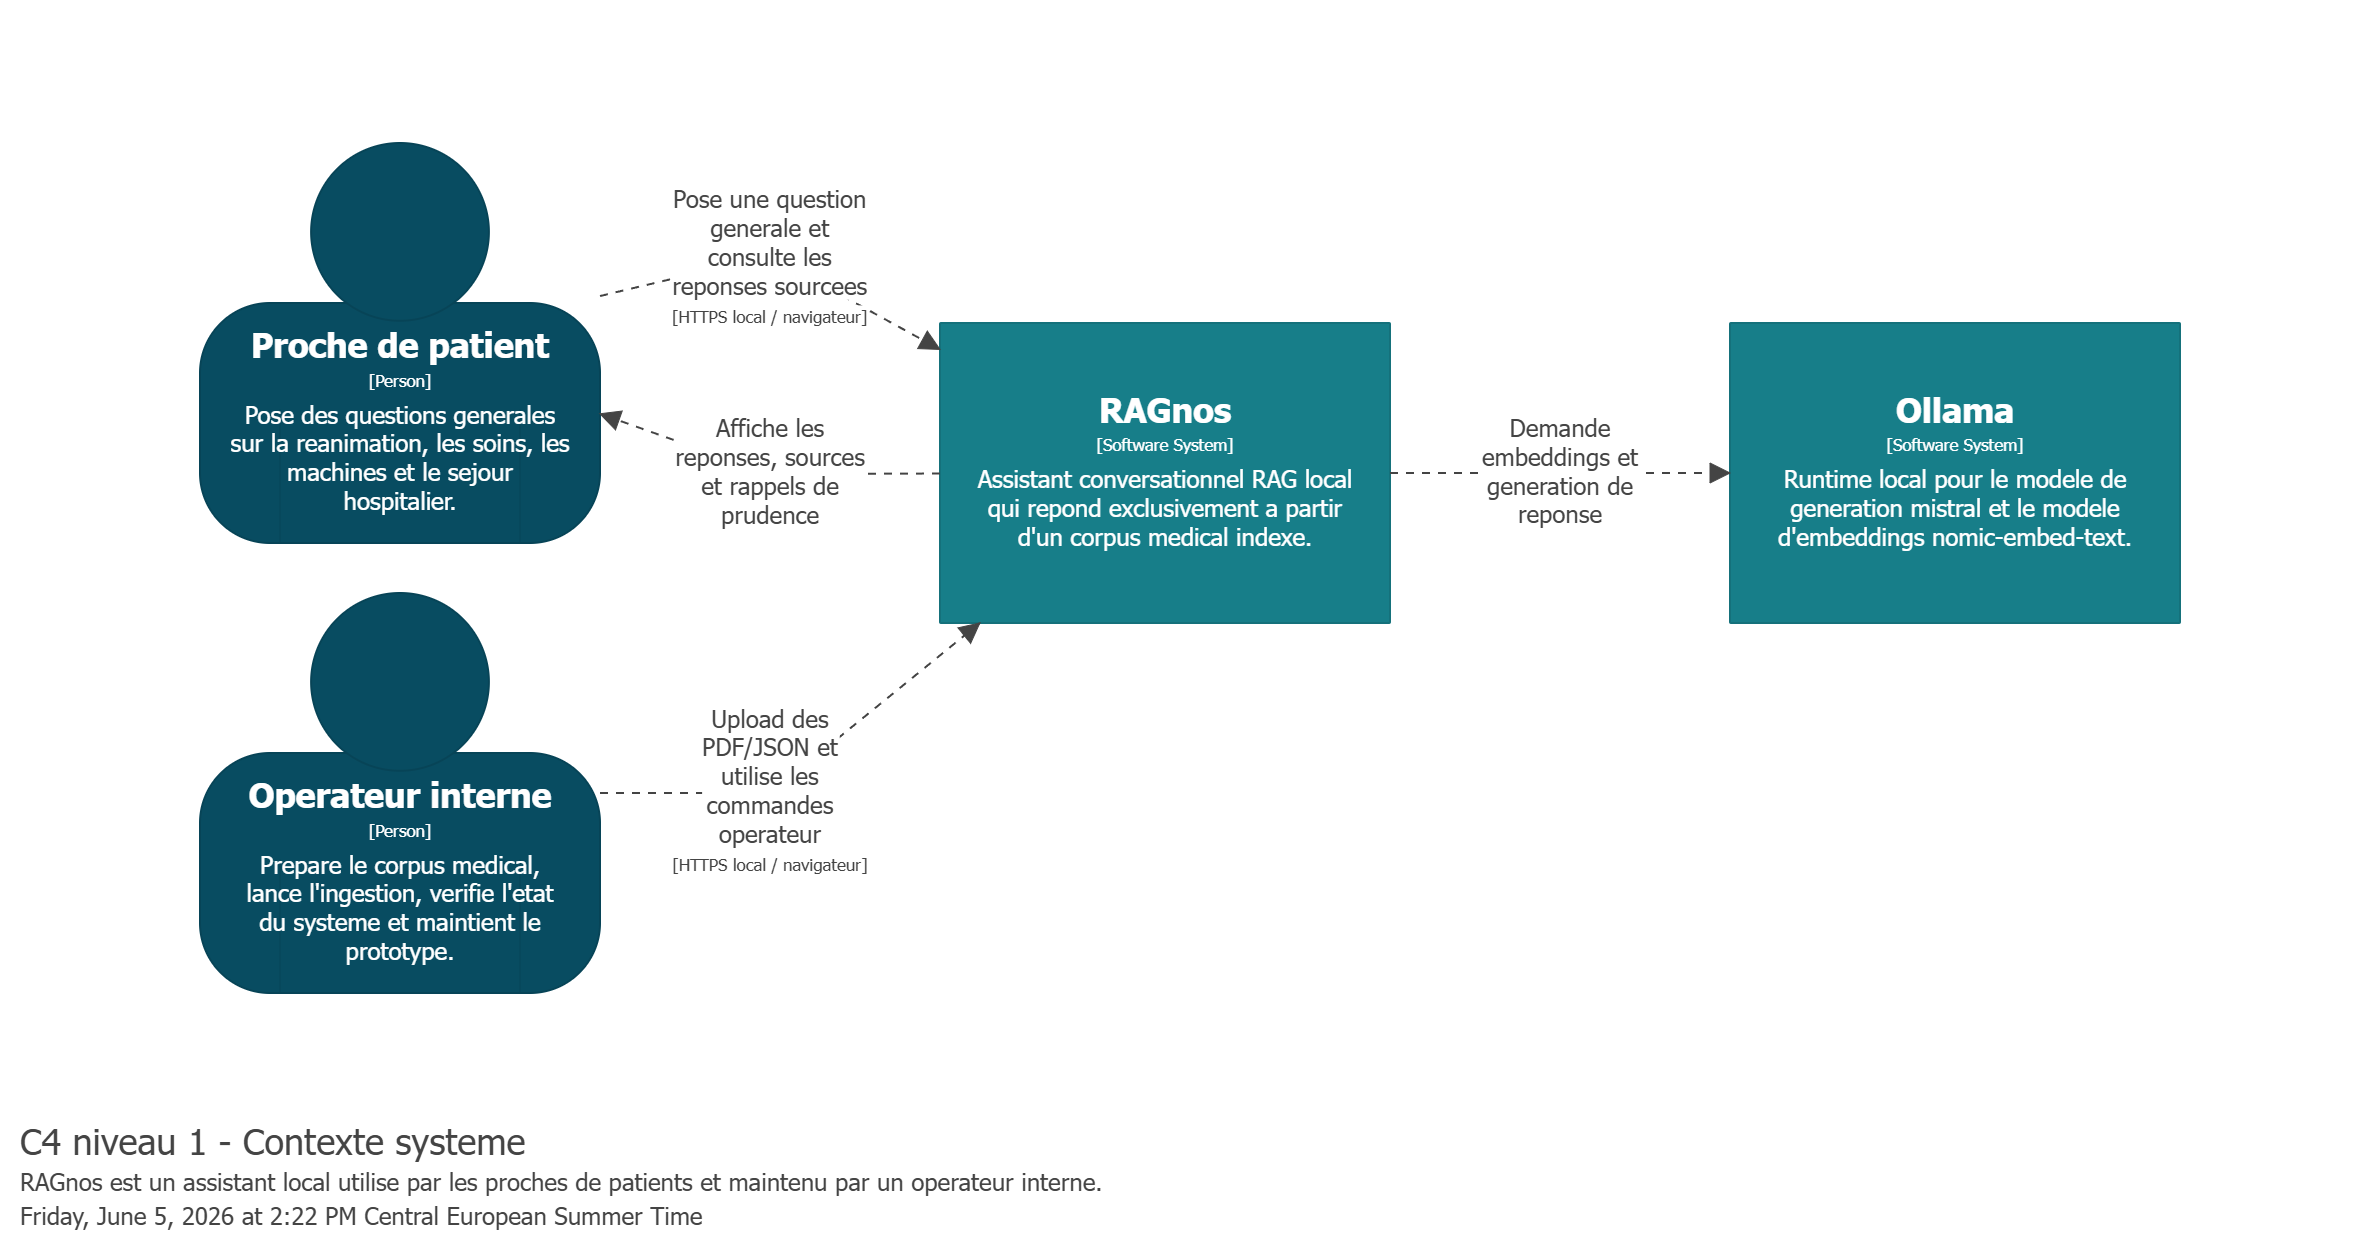
\includegraphics[width=\textwidth,height=0.68\textheight,keepaspectratio]{SystemContext.png}
  \caption{Vue C4 niveau 1 : contexte systeme de RAGnos pour l'information en reanimation.}
  \label{fig:c4-system-context}
\end{figure}

\begin{figure}[htbp]
  \centering
  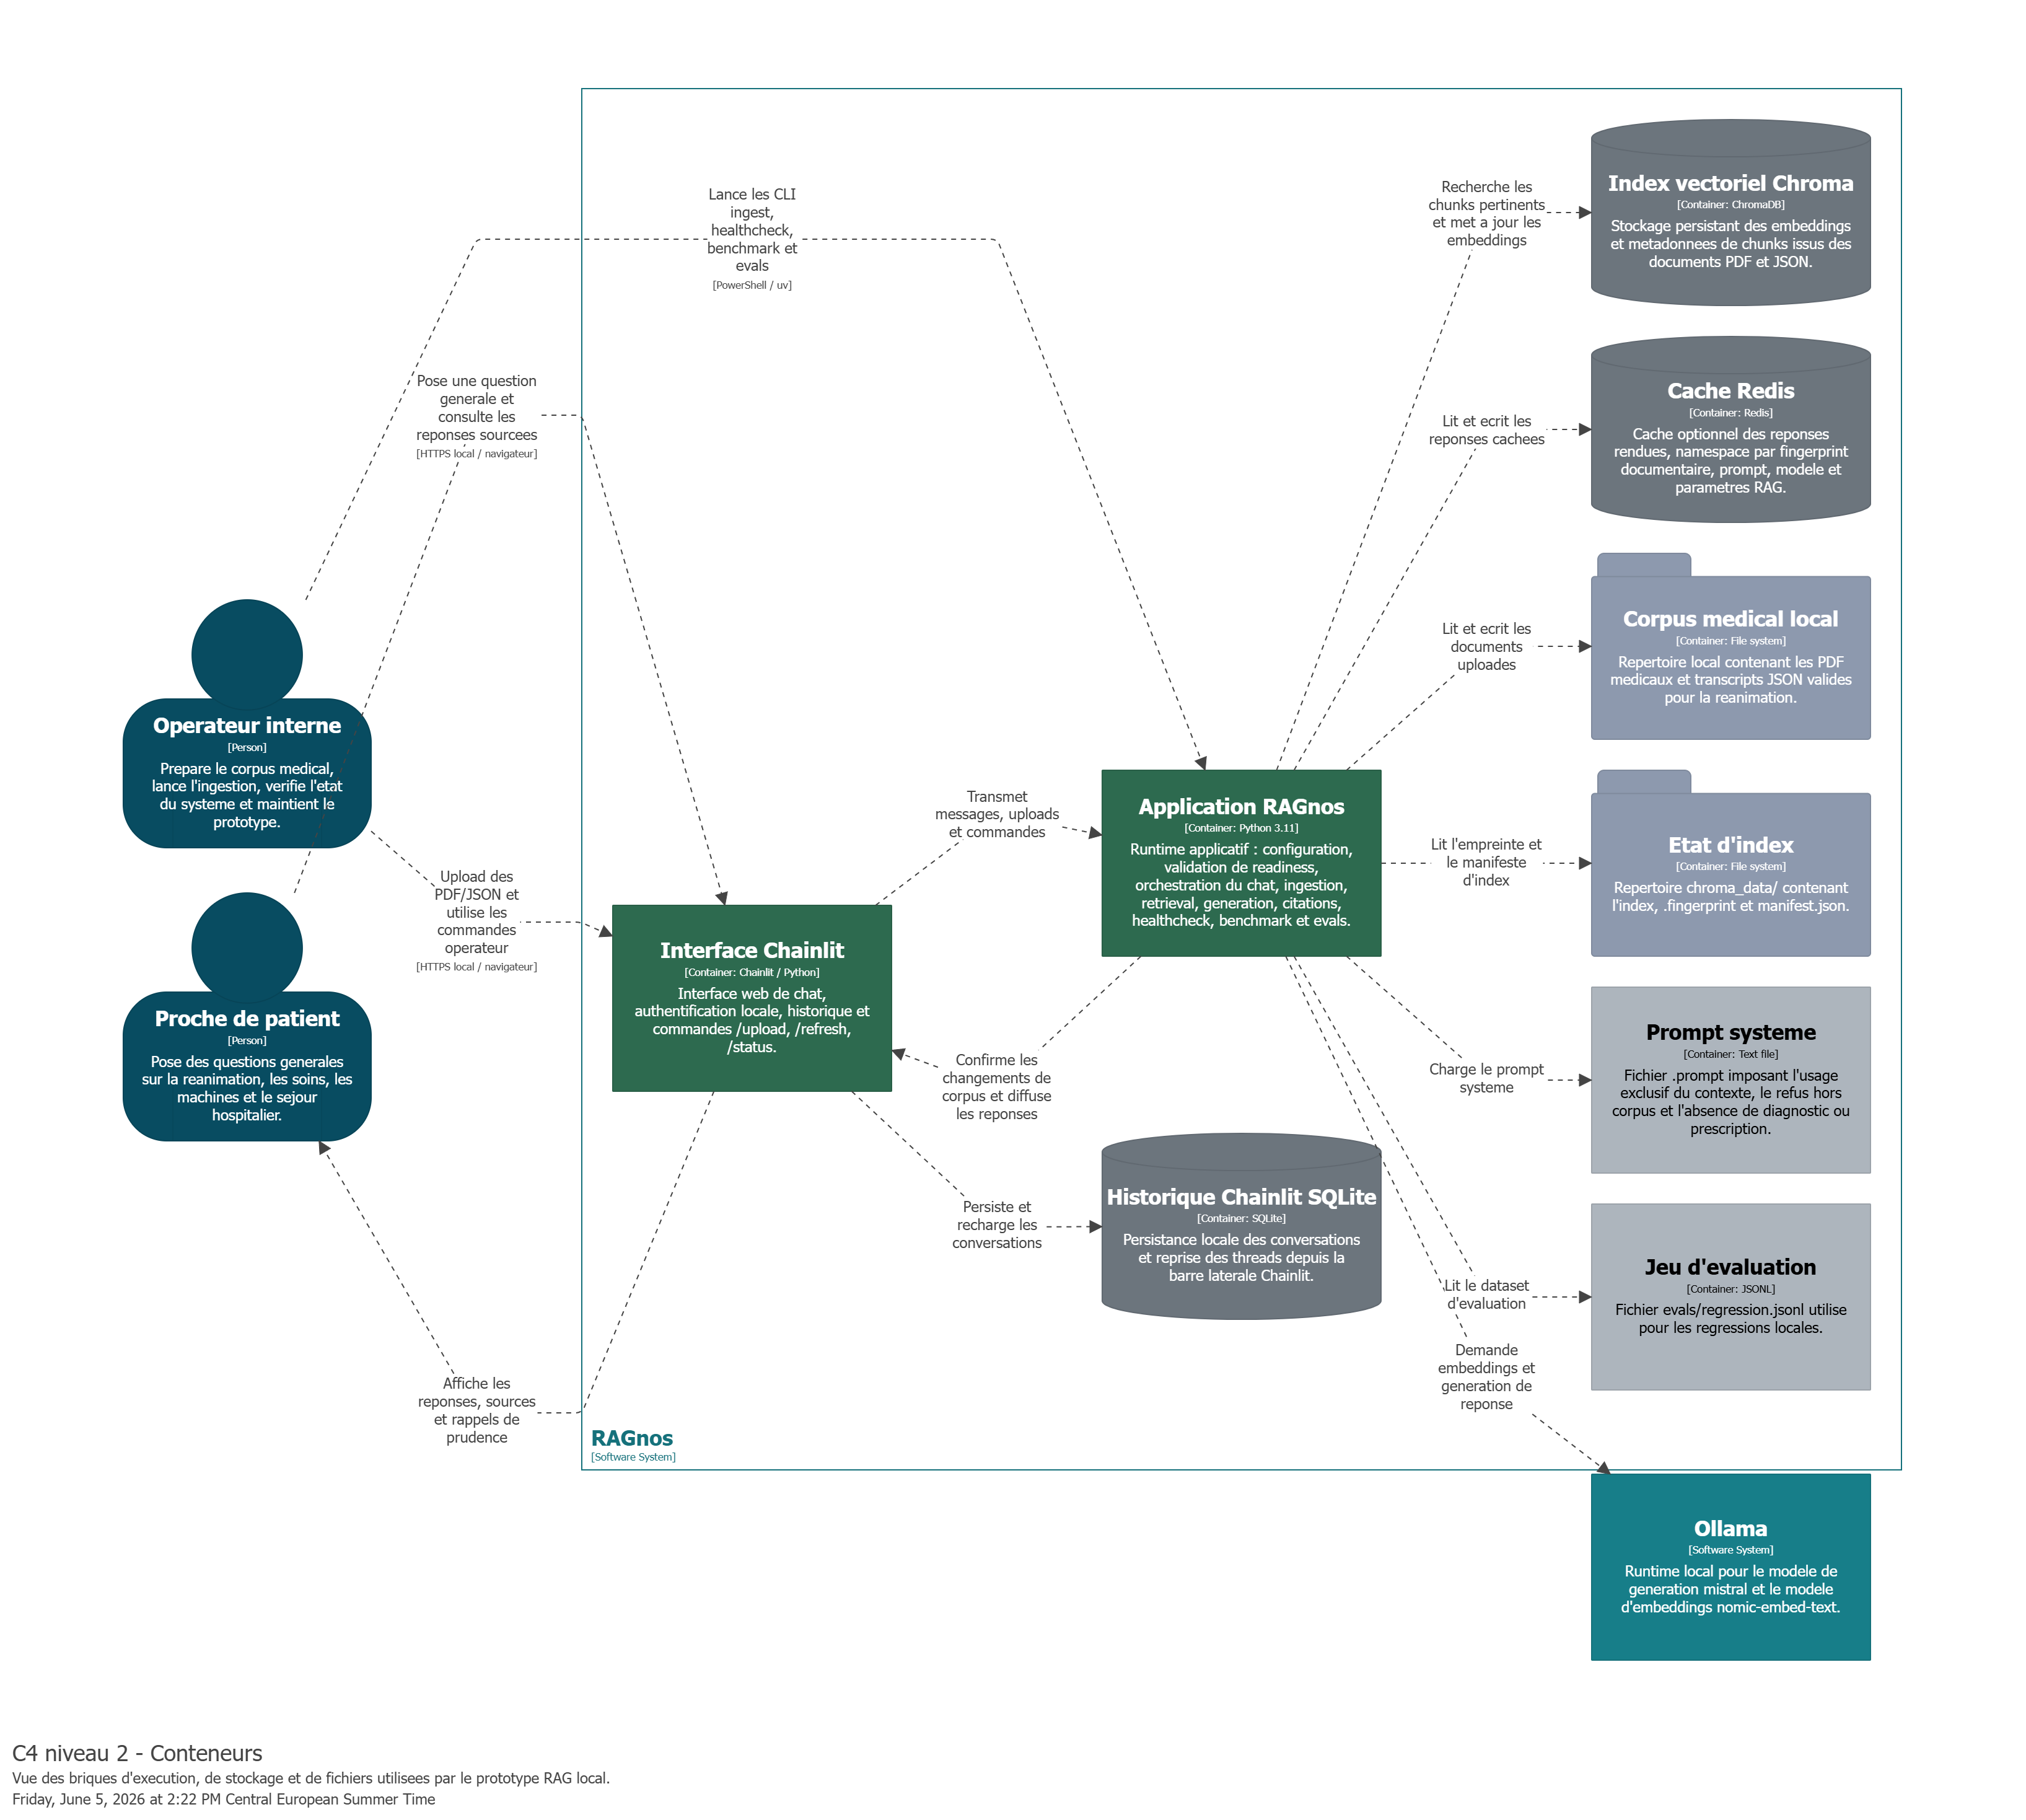
\includegraphics[width=\textwidth,height=0.68\textheight,keepaspectratio]{Containers.png}
  \caption{Vue C4 niveau 2 : conteneurs techniques du prototype local.}
  \label{fig:c4-containers}
\end{figure}

\begin{figure}[htbp]
  \centering
  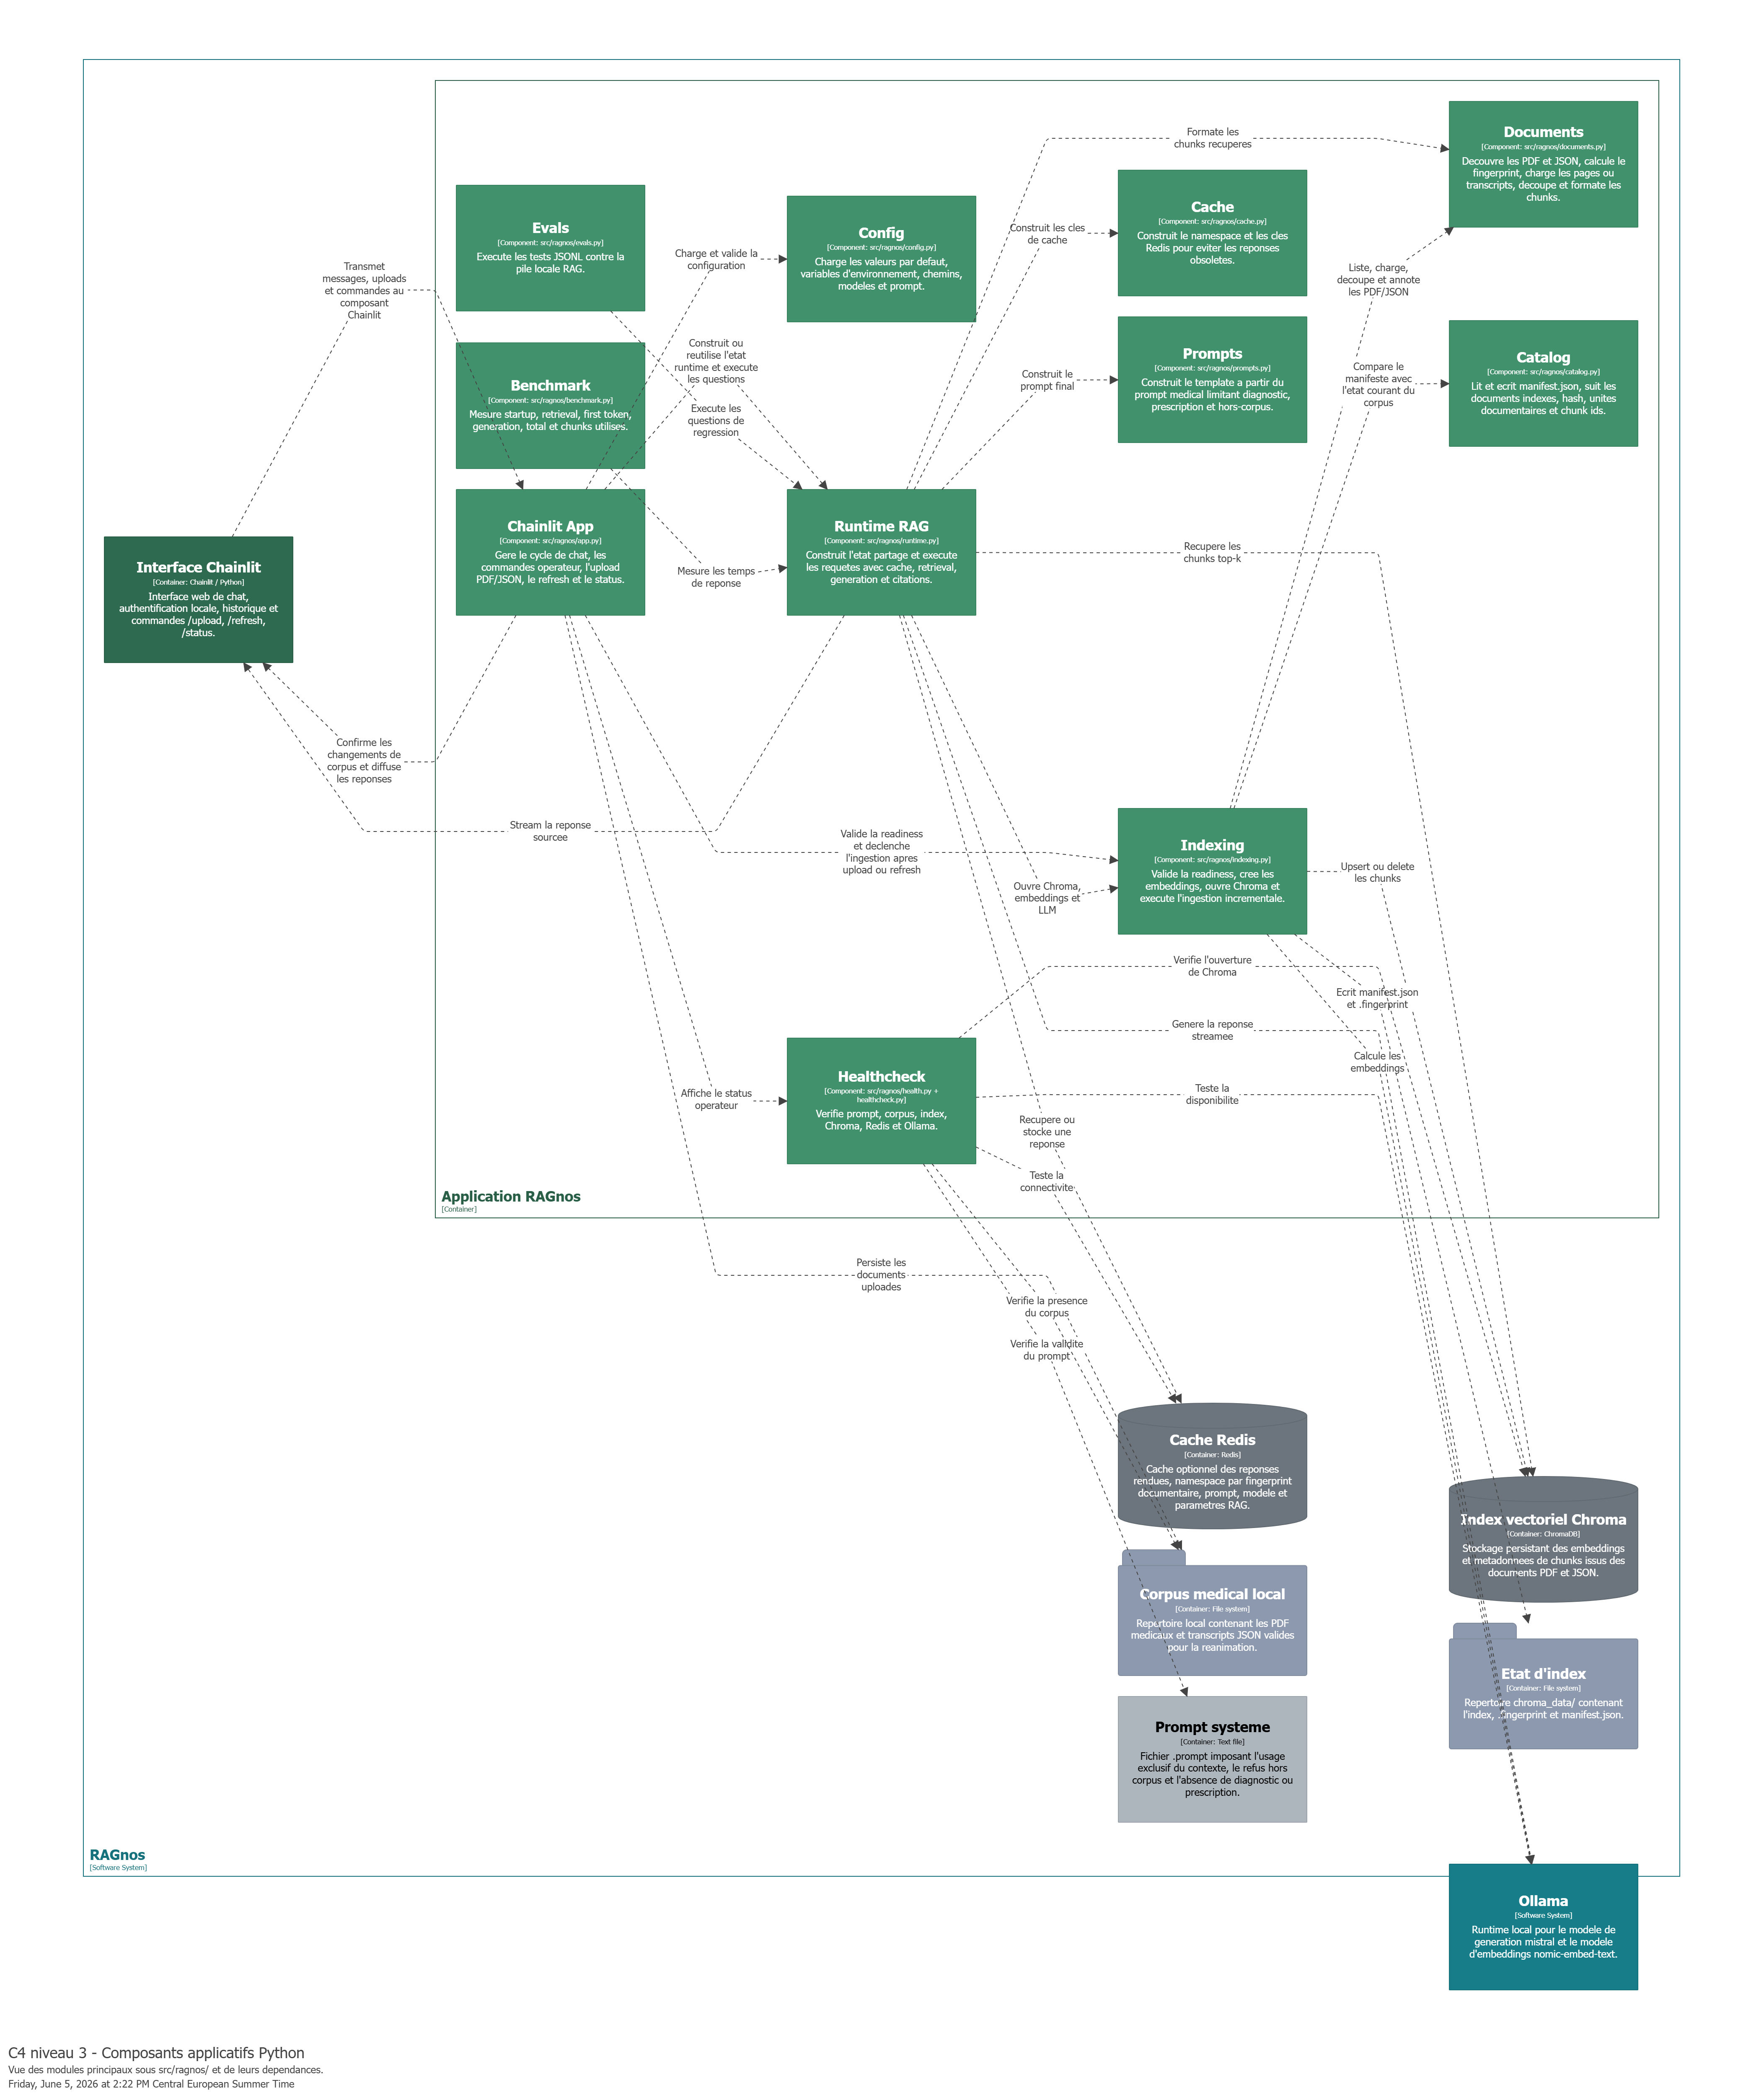
\includegraphics[width=\textwidth,height=0.72\textheight,keepaspectratio]{Components.png}
  \caption{Vue C4 niveau 3 : composants applicatifs Python de RAGnos.}
  \label{fig:c4-components}
\end{figure}

\subsection{Ingestion}

Le pipeline d'ingestion decouvre les fichiers \texttt{.pdf} et \texttt{.json}, calcule une empreinte de corpus, charge les documents, les decoupe en chunks, cree les embeddings et met a jour Chroma. Les fichiers JSON de transcripts sont charges comme documents textuels avec metadonnees, tandis que les PDF sont charges page par page. Cette evolution correspond directement au nouveau corpus medical.

L'ingestion reste incrementale : les fichiers inchanges sont evites, les fichiers modifies sont reindexes et les fichiers supprimes voient leurs chunks retires de l'index.

\begin{figure}[htbp]
  \centering
  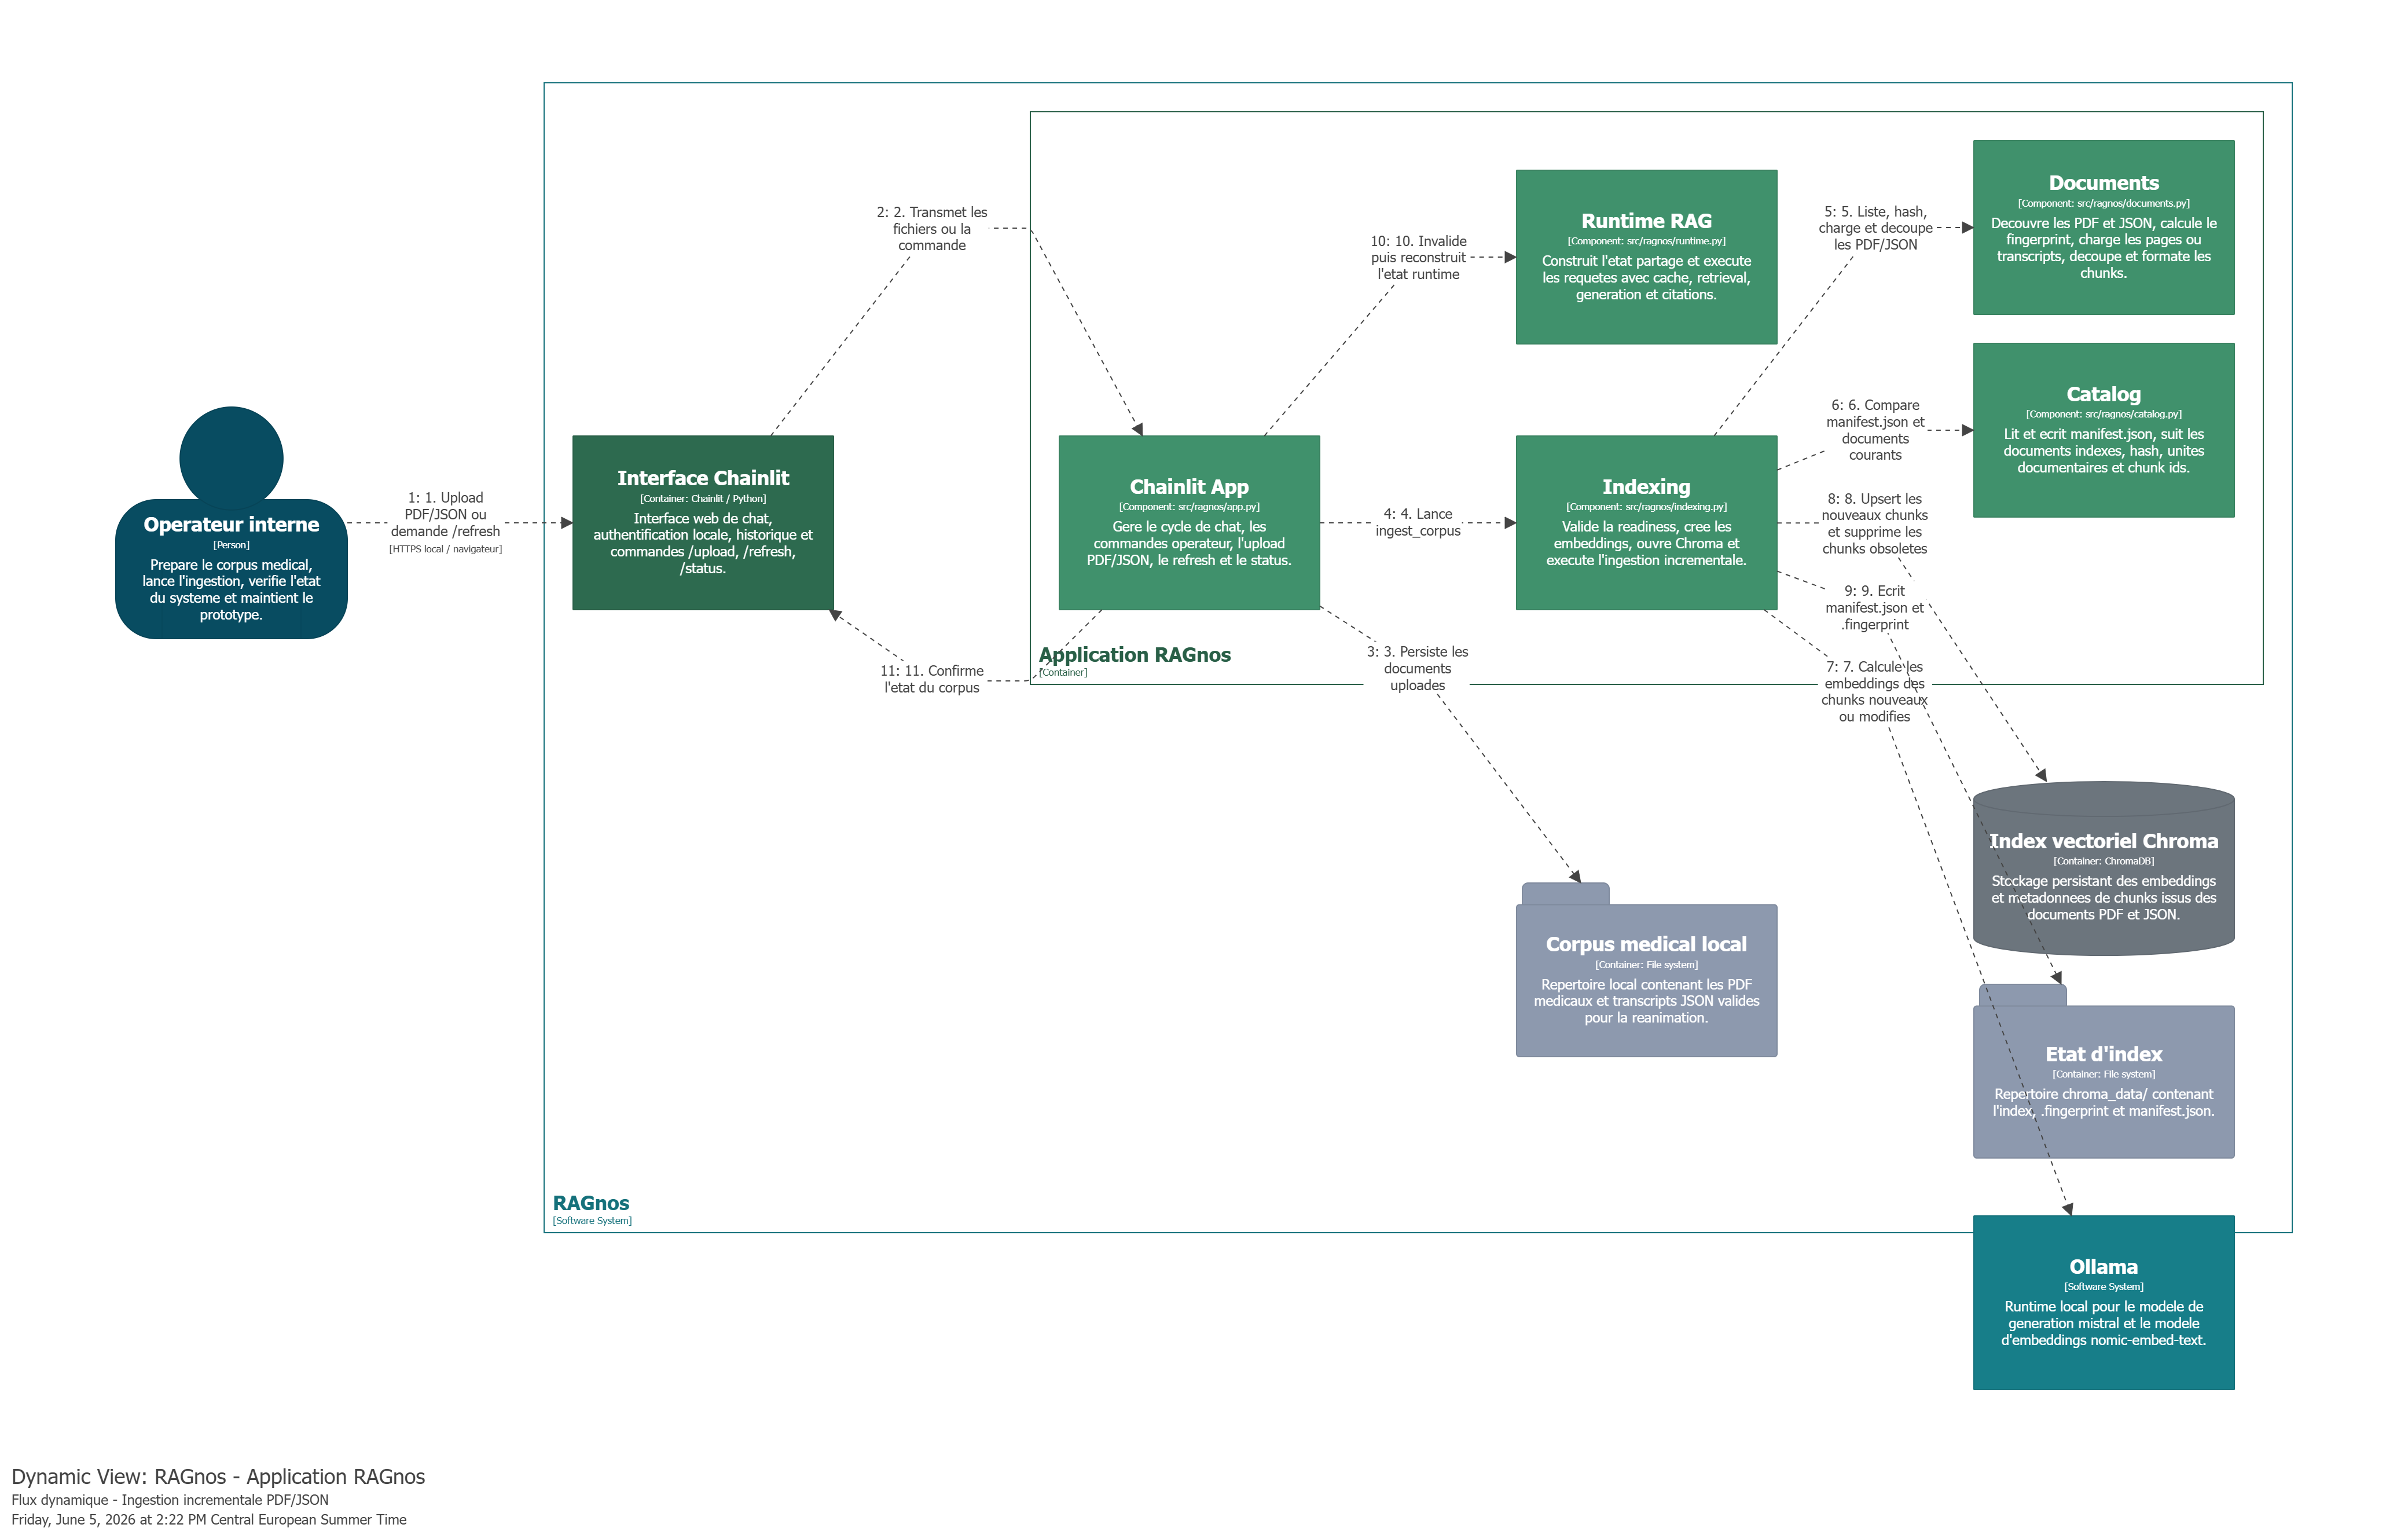
\includegraphics[width=\textwidth,height=0.68\textheight,keepaspectratio]{IngestFlow.png}
  \caption{Vue dynamique C4 : ingestion incrementale du corpus PDF et JSON.}
  \label{fig:c4-ingest-flow}
\end{figure}

\subsection{Requete}

Lorsqu'un utilisateur pose une question, RAGnos suit le chemin suivant :

\begin{enumerate}
  \item recuperation des chunks les plus proches dans Chroma ;
  \item formatage du contexte avec nom de fichier et page ou section transcript ;
  \item appel du LLM local avec le prompt medical ;
  \item ajout d'un bloc \texttt{Sources:} construit par le code ;
  \item mise en cache eventuelle de la reponse.
\end{enumerate}

Cette architecture est suffisante pour un prototype. Pour un usage plus robuste, les priorites sont : retrieval hybride, reranking, seuil de pertinence, evaluation de groundedness et meilleure granularite des citations.

\begin{figure}[htbp]
  \centering
  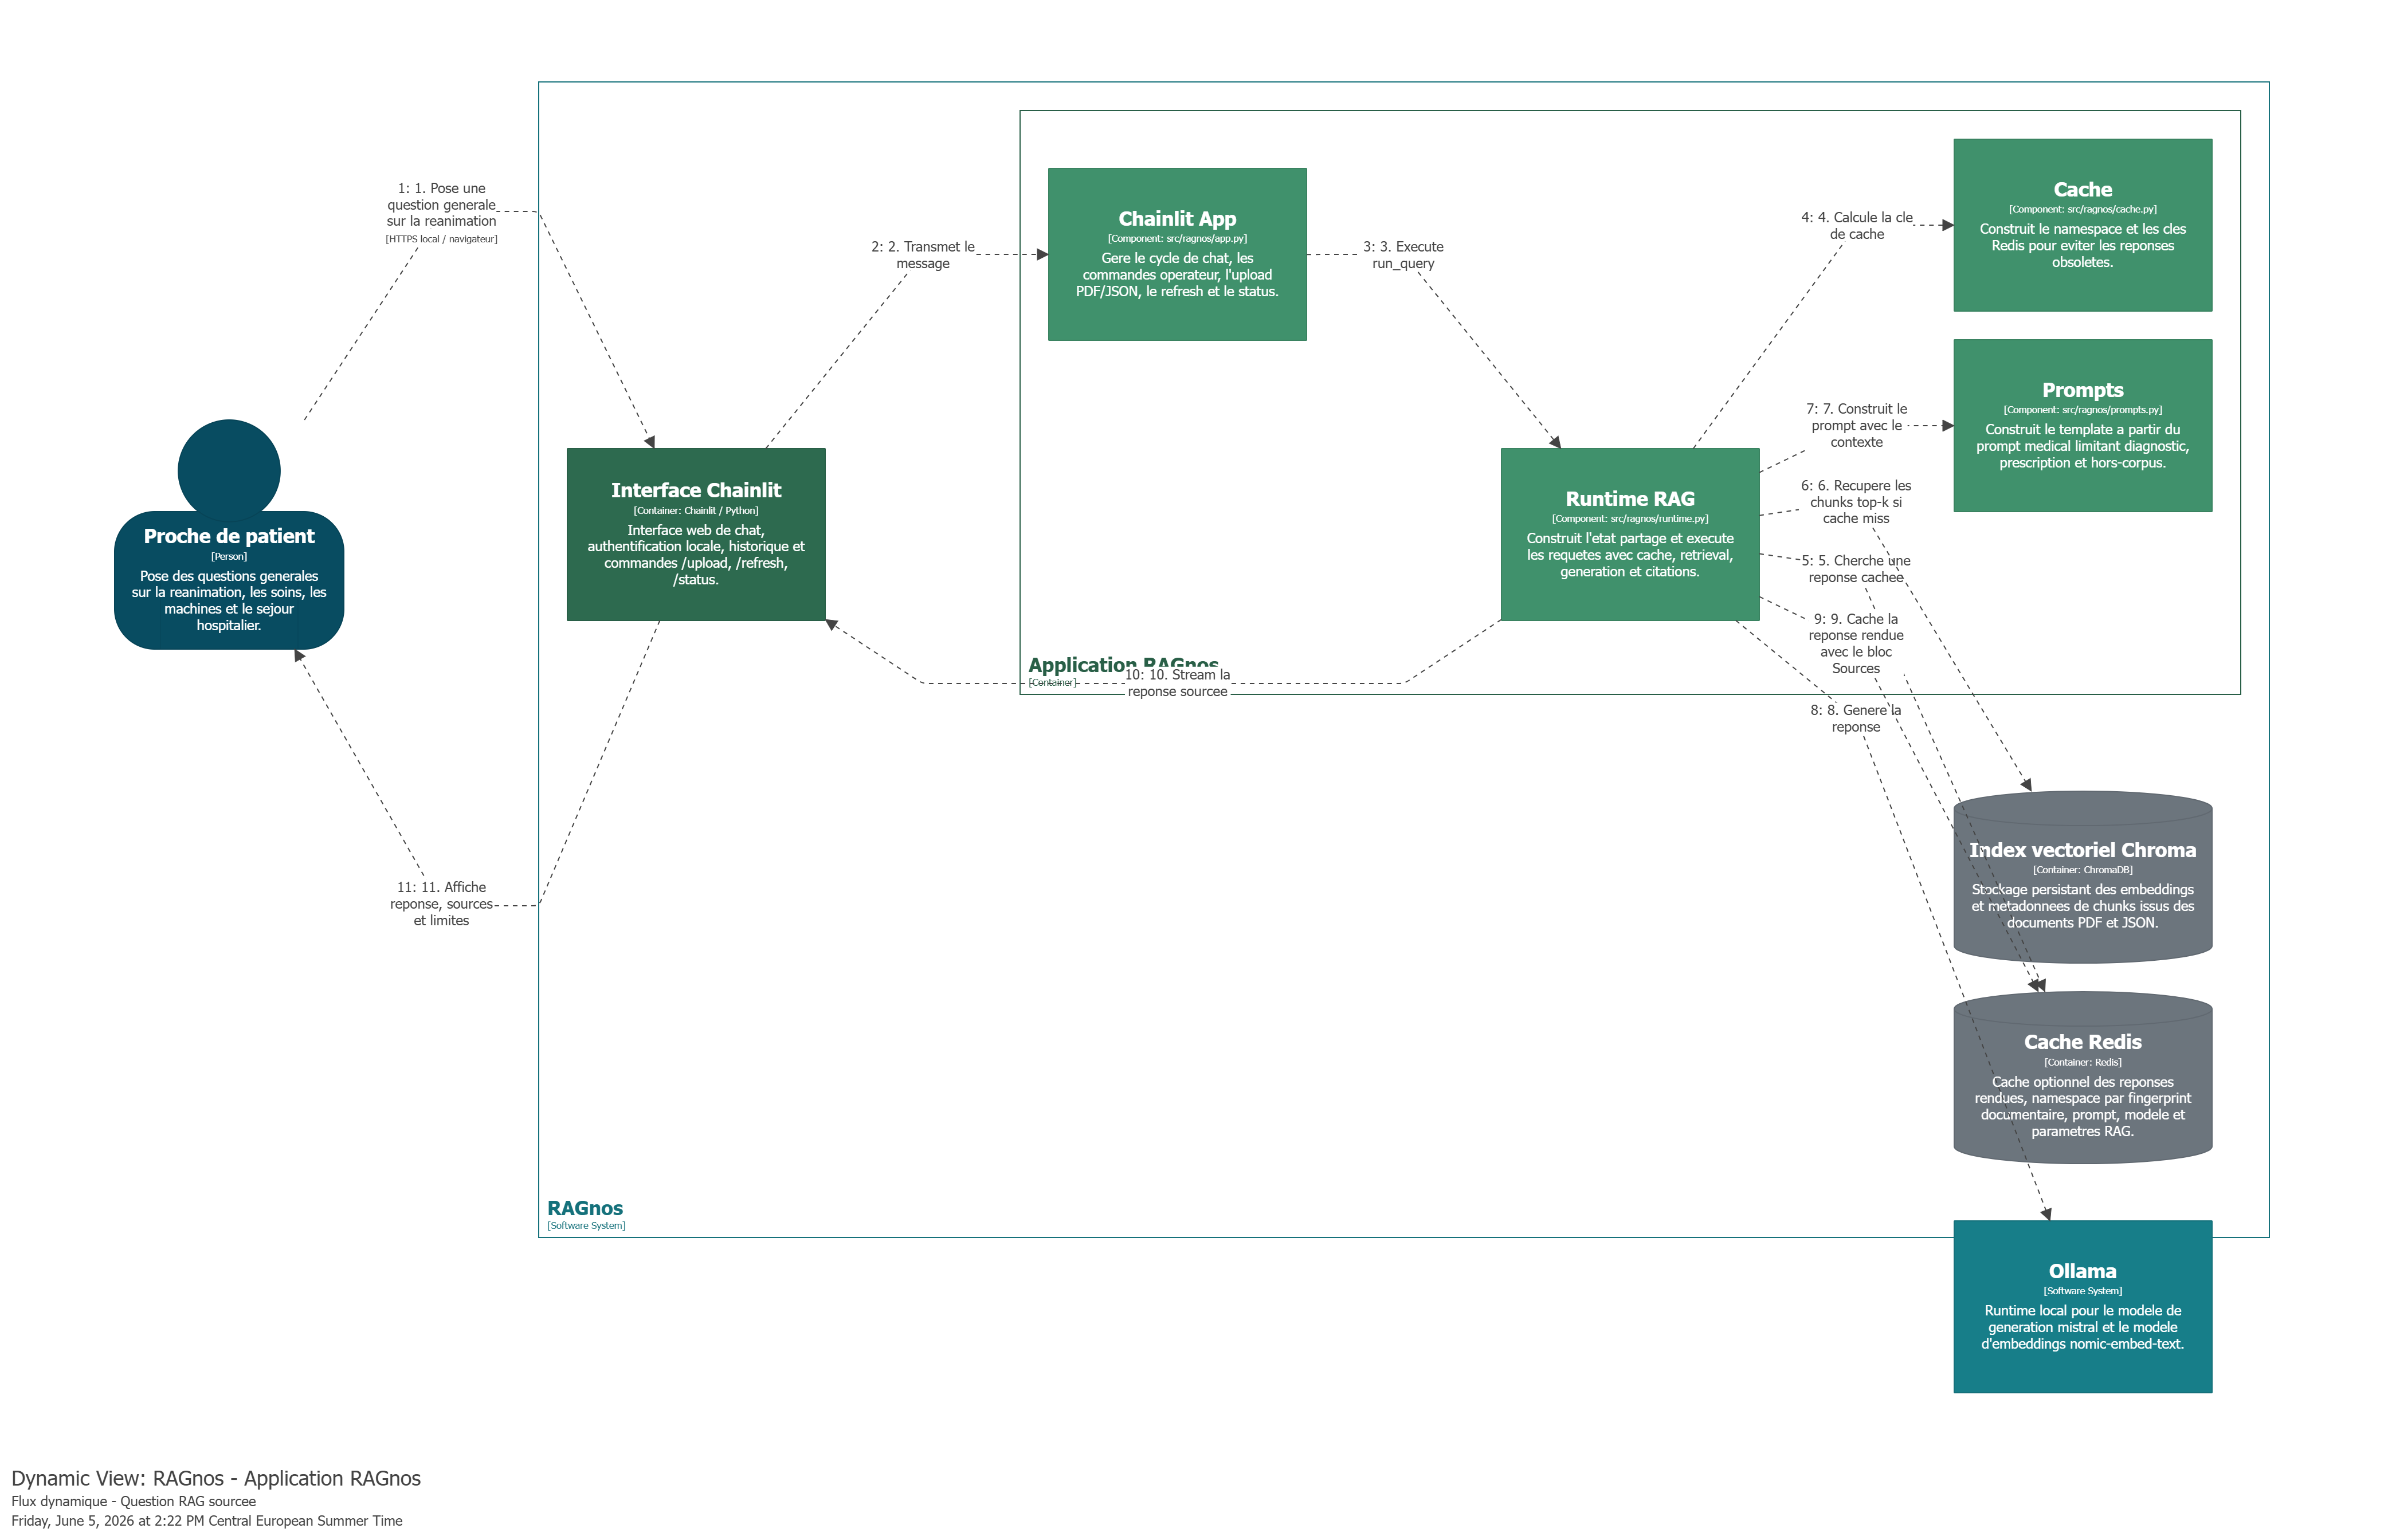
\includegraphics[width=\textwidth,height=0.68\textheight,keepaspectratio]{QueryFlow.png}
  \caption{Vue dynamique C4 : traitement d'une question sourcee.}
  \label{fig:c4-query-flow}
\end{figure}

\section{Evaluation}

Une evaluation serieuse doit depasser l'exactitude brute. MultiMedQA couvre des questions medicales de differents publics et utilise des evaluations humaines ; Med-HALT cible specifiquement les hallucinations medicales ; des benchmarks de long-form medical QA integrent correctness, helpfulness, harmfulness et biais \autocite{multiMedQA,medHalt,longFormMedicalQA}.

Pour RAGnos, les criteres d'evaluation pertinents sont :

\begin{itemize}
  \item presence de la bonne source ;
  \item absence d'information hors corpus ;
  \item refus correct en cas d'absence de source ;
  \item comprehensibilite pour des non-specialistes ;
  \item ton prudent et adapte ;
  \item absence de diagnostic ou prescription ;
  \item distinction claire entre information generale et cas individuel.
\end{itemize}

Pour l'information aux proches, les outils d'evaluation de litteratie en sante sont particulierement utiles. Le PEMAT de l'AHRQ et le CDC Clear Communication Index permettent d'evaluer la comprehension et l'actionnabilite, ce qui est plus adapte a un public non specialiste que des mesures purement cliniques \autocite{ahrqPEMAT,cdcClearCommunication}.

\section{Limites et ameliorations prioritaires}

\subsection{Limites actuelles}

Le prototype reste volontairement limite. Il ne garantit pas la justesse clinique d'une reponse, ne verifie pas automatiquement l'actualite d'une source, ne classe pas encore les documents par niveau de preuve et ne mesure pas la groundedness proposition par proposition. Il n'implemente pas encore la recherche hybride ni le reranking.

Ces limites ne rendent pas le projet inutile. Elles delimitent son usage defendable : un assistant pedagogique local pour information generale, pas un outil de decision medicale.

\subsection{Priorites}

Les ameliorations les plus utiles sont :

\begin{enumerate}
  \item ajouter un refus deterministe si aucun chunk pertinent n'est recupere ;
  \item ajouter un seuil de pertinence minimal ;
  \item implementer une recherche hybride BM25 + embeddings ;
  \item ajouter un reranker leger ;
  \item enrichir les metadonnees documentaires ;
  \item construire un jeu d'evaluation medical avec questions positives, negatives et sources attendues ;
  \item evaluer les reponses avec des criteres de comprehension pour proches non specialistes ;
  \item ajouter une commande \texttt{/list} pour afficher les documents indexes.
\end{enumerate}

\section{Lien avec l'ancien cadrage juridique}

Le projet RAGnos etait initialement centre sur la consultation juridique. Cette matiere a ete sortie du rapport principal et conservee dans une annexe autonome : \path{docs/annexe_etat_art_juridique.tex}. Elle reste utile comme historique, car le domaine juridique partage avec le medical des exigences fortes de sources, de refus, de tracabilite et de validation humaine.

Le rapport principal doit cependant etre lu comme un rapport medical. Le cas d'usage, le corpus, le prompt, les risques et les perspectives sont desormais ceux de la reanimation et de l'information aux proches.

\section{Conclusion}

RAGnos ne doit pas chercher a devenir un assistant clinicien. Sa valeur reside dans un perimetre plus strict : expliquer clairement des informations generales de reanimation a partir de sources validees, afficher les sources, refuser lorsque le corpus ne permet pas de repondre et rappeler que l'equipe soignante reste seule competente pour le cas individuel \autocite{sccmFamilyCentered2024,sfarInfoPatientsRea,euAIActHealthcare}.

Ce positionnement est techniquement coherent avec une architecture RAG locale et medicalement plus defendable qu'un chatbot generaliste. Les evolutions attendues concernent le retrieval, les metadonnees, l'evaluation, les refus et la qualite du corpus afin de rapprocher le prototype d'un outil fiable d'information aux proches.

\printbibliography

\end{document}
